\documentclass[a4paper]{article}
\usepackage{amsmath}
\usepackage{amsthm}
\usepackage[left=1.8cm,right=1.8cm,top=2.2cm,bottom=2.0cm]{geometry}
\usepackage{enumerate}
\usepackage{fancyhdr}
\usepackage{xpatch}
\usepackage{graphicx}
\usepackage{float}
\usepackage{subfigure}
\usepackage{amsfonts}
\usepackage{mathtools}
\usepackage{framed}
\usepackage{multicol}
\usepackage{fontspec}
\usepackage{float}
\usepackage{algpseudocode}
\usepackage{extarrows}
\usepackage{algorithm}
\usepackage{tikz}
\usepackage{caption}
\makeatletter

\printanswers


\AtBeginDocument{\xpatchcmd{\@thm}{\thm@headpunct{.}}{\thm@headpunct{}}{}{}}
\makeatother

\pagestyle{fancy}
\renewcommand{\baselinestretch}{1.15}
\newcommand{\code}[1]{\texttt{#1}}
\usepackage{paralist}
\let\itemize\compactitem
\let\enditemize\endcompactitem
\let\enumerate\compactenum
\let\endenumerate\endcompactenum
\let\description\compactdesc
\let\enddescription\endcompactdesc

% shorten footnote rule
\xpatchcmd\footnoterule
  {.4\columnwidth}
  {1in}
  {}{\fail}

\title{CSE 220 Final}
\author{\textbf{Yiwei Yang} \\ \texttt{ yyang363@ucsc.edu}}


\begin{document}
\maketitle
\section{}

\subsection{}
$f(n)=\omega(g(n))$
\subsection{}
$f(n)=o(g(n))$
\subsection{}
$f(n)=\Theta(g(n))$
\subsection{}
$f(n)=\Theta(g(n))$
\subsection{}
$f(n)=\Theta(g(n))$
\section{}
\subsection{}

\begin{proof}
  Weak Induction:

  The base case $n=1$ $LHS=\sum_{i=1}^n \mathrm{~F}(\mathrm{i})^2=F(1)=1, RHS= \mathrm{F}(\mathrm{n})^* \mathrm{~F}(\mathrm{n}+1)=F(1)*F(2)=1*1=1$
  
  Suppose the case for $n=k> 1$ $\sum_{i=1}^k \mathrm{~F}(\mathrm{i})^2=\mathrm{F}(\mathrm{k})^* \mathrm{~F}(\mathrm{k}+1)$ is correct, we have when $n=k+1$, $\sum_{i=1}^{k+1} \mathrm{~F}(\mathrm{i})^2=\mathrm{F}(\mathrm{k})^* \mathrm{~F}(\mathrm{k}+1)+F(k+1)^2=F(k+1)*(F(k)+F(k+1))=F(k+1)F(k+2)= \mathrm{F}(\mathrm{k+1})^* \mathrm{~F}(\mathrm{k}+2)$
\end{proof}

\subsection{}
\begin{proof}
  2 variable Weak Induction:
  
  The base case, $i=0$, we have $A(0,j)=j+1>j$ follows
  
  Induction Hypothesis: from $i$ to $i+1$, $i\geq 0$, use the induction to prove for some $i$ s.t. for all $j$, $A(i,j)>j$
  \begin{enumerate}
    \item Base case: $j=0$, $A(i+1,0)=A(i,1)>1>0$.
    \item Induction hypothesis: we observe that the function is discrete, so we can use if $m>n$ then $m\geq n+1$, we have $A(j+1,i+1)=A(i,A(i+1,j))\geq A(i+1,j)+1\geq(j+1)+1>j+1$
  \end{enumerate}

\end{proof}

\section{}
\subsection{}
Since given $f(n)=n^2 log(n)$, $f(n)=\Omega(n^{log_36+\epsilon})$,we have $6f(n/3)\leq cf(n)$, with constant $c<1$, it's in case 3.

We have $T(n)=\Theta\left(n^2 \log n\right)$
\subsection{}
Since given $f(n)=n^2$, $f(n)=\Omega(n^{log_20.5+\epsilon})$,we have $0.5f(n/2)\leq cf(n)$, with constant $c<1$, it's in case 3.

We have $T(n)=\Theta\left(n^2 \right)$
\subsection{}
Since given $f(n)= n$, we have $f(n)=O(n^{log_23-\epsilon})$, it's in case 1

We have $T(n)=\Theta\left(n^{\lg 3}\right)$
\subsection{}
Since given $f(n)= nlog(n)$, we have $f(n)=\Omega(n^{log_33+\epsilon})$,we have $3f(n/3)\leq cf(n)$, with constant $c<1$, it's in case 3.

We have $T(n)=\Theta\left(n \log n\right)$

\section{}
\begin{proof}
  We can seen by drawing the graph generated by recurrence $T(n)=\sum_{i=0}^{\log _b n} a^i f\left(n / b^i\right)+O\left(n^{\log _b a}\right)$, where $f(n)=cn^d, a\geq 1, b>1$
  \\
  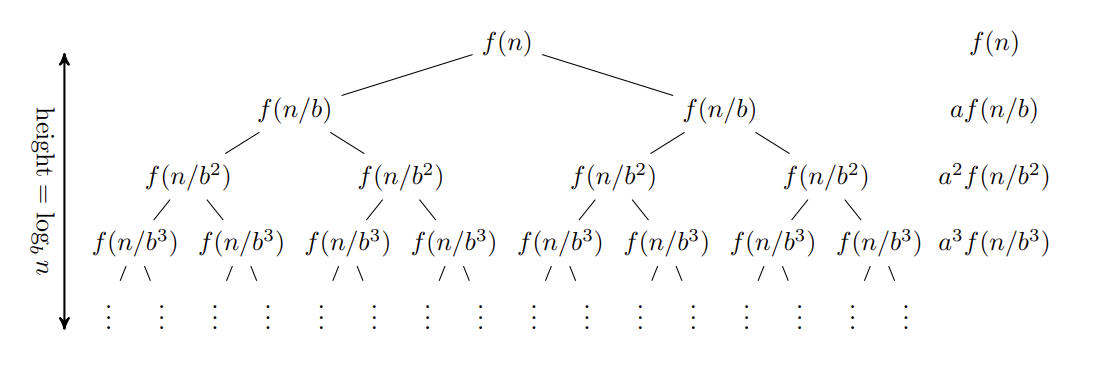
\includegraphics[width=\textwidth]{test.png}

  The total work for the tree is $\sum_{i=0}^{\log _b n} a^i f\left(n / b^i\right)=c\cdot n^d \cdot \sum_{i=0}^{\log _b n} (\frac a{b^d})^i$. we have if $a<b^d$, the complexity dominated by the initial work at the root, and we have $T(n)=O(n^d)$
\end{proof}

\section{}

\subsection{}

The input is set $G$ repersenting Green jugs and $P$ repersenting Purple jugs, both of them are in set 1-n and their size are obviously the same 
\begin{algorithm}
  \caption{MATCH-JUGS$(G,P)$}\label{alg:cap3}
  \begin{algorithmic}[1]
    \If{$|G|=0$}
    \State{return}
    \EndIf
    \If{$|G|=1$}
    \State{$G=\{g\}$}
    \State{$P=\{p\}$}
    \State{return}
    \Else
    \State{choose random g from set $G$}
    \State{$G_{smaller}=$ the set of smaller jugs than $g$ in G
    \State{$G_{larger}=$ the set of larger jugs than $g$ in G
    \State{$p=$ find\_if(P.begin(),P.end(),[](jug a)\{return a.water==g;\})}

    \State{$P_{smaller}=$ the set of smaller jugs than $p$ in P
    \State{$P_{larger}=$ the set of larger jugs than $p$ in P
    \State{MATCH-JUGS$(G_{smaller},P_{smaller})$}
    \State{MATCH-JUGS$(G_{larger},P_{larger})$}
    \EndIf
  \end{algorithmic}
\end{algorithm}

The correctness is easy, similar to quicksort, we can pick random pivot from $G$ and get the same pivot in $P$, we ca
 And like wise between the jugs larger than $g$. Termination is also easy to see: Since $\left|G_{smaller}\right|+\left|G_{greater}\right|<|G|$ in every recursive step, the size of the first parameter reduces with every recursive call. It eventually must reach 0 or 1 , in which case the recursion terminates.

 The worst case running time of above algorithm is in $\Theta(n^2)$. Say we can get the recurrence for MATCH-JUGS worst case time is 

 $$T(n)=\max _{0 \leq q \leq n-1}(T(q)+T(n-q-1))+\theta(n)$$ The partition is q, we can simply prove that $\mathrm{T}(\mathrm{n})=\Omega\left(\mathrm{n}^2\right)$ using $\mathrm{n}+(\mathrm{n}-1)+\ldots+2+1=\sum_{i=1}^{n-1} i=\mathrm{n}^*(\mathrm{n}+1) / 2=\Omega\left(\mathrm{n}^2\right)$.
 
 Then we prove $T(n)=O(n^2)$ using substitution method. guess $\mathrm{n}+(\mathrm{n}-1)+\ldots+2+1=\sum_{i=1}^{n-1} i=\mathrm{n}^*(\mathrm{n}+1) / 2=\Omega\left(\mathrm{n}^2\right) $ for const $c$:

 \begin{enumerate}
  \item Base Case: $T(n)\leq c$
  \item Strong backward induction: $$\begin{aligned}
    & \mathrm{T}(\mathrm{n}) \leq \max _{0 \leq q \leq n-1}\left(c q^2+c(n-q-1)^2\right)+\theta(n) \\
    & \mathrm{T}(\mathrm{n})=c \max _{0 \leq q \leq n-1}\left(q^2+(n-q-1)^2\right)+\theta(n)
    \end{aligned}$$
    Using derivative we knows that the mas is when $q=0/q=n-1$, thus $ \mathrm{T}(\mathrm{n}) \leq c(n-1)^2+\theta(n)=c *\left(n^2-2 n+1\right)+\theta(n) \leq \mathrm{cn}^2$
 \end{enumerate}
So $T(n)\leq cn^2$, thus $T(n)=O(n^2)$, thus $T(n)=\Theta(n^2)$.
\subsection{}
Since this is very similar to quick sort, which is devide and conquer, we can know that by theory, we have to satisfy the height of the decision tree $h\geq\lceil log_kz\rceil$, where k is the k-ary tree and z is the number of leaves. 

Let $x$ be the maximum number of comparisons in a sorting algorithm. The maximum height of the decision tree would be x. A tree with maximum height x has at most $2^x$ leaves.

Thus we have $x\geq log_2(n!)=\Omega(n log n)$. Thus any algorithm's time complexity will be $\Omega(n log n)$

\section{}
\subsection{}
$T(n)=n * \log k+k * T(n / k)$

\subsection{}
Since given $f(n)=n log(k)$, $f(n)=\Theta(n^{log_kk+\epsilon})$, it's in case 2.

We have $T(n)=\Theta(nlogn)$

\section{}
\subsection{}
The optimal substructure is first computing the length of longest decreasing subsequence of the subarray A[1:j], for calculating the $L[j]$, the longest decrasing subsequence of all the prev number should comply $A[j]\geq A[i]$ for $j<i$ and if found, just let $L[i]$ to be the $max\{L[j]\} +1$
\subsection{}
Let optimal substructure 
$$L[i]\left\{\begin{array}{l}
  1+max\{L[j]\}, \text{ when at least on j such that } j<1\text{ and } A[j]\geq A[i]\\
  1, \text{ when there's no such j}
}\end{array}\right$$

To proof the currectness, first we have base case $L[1]=1$, the recurrence is currect because the coutcome is decreasing weakly subsequence if you put $A[i]$ after a sequence that ends with $A[j]$, iff $A[j]\geq A[i]$ and $j<i$ and the longest weakly sequence will be +1, for any other cases, we just get 1 is okay.

\subsection{}

\begin{algorithm}
  \caption{LongestWeaklyDecreasing$(arr,n)$}\label{alg:cap3}
  \begin{algorithmic}[1]
    \For{$i=1..n$}
    \State{$maxlen=1$}
    \State{$L[i]=1$}
    \For{$j=1..i-1$}
    \If{$A[j]>=A[i]$}
    \State{$L[i]=max\{L[i],L[i]+1\}$}
    \EndIf
    \EndFor
    \EndFor
    \State{return $max\{L[j]\}$ where the weakly minimun is taken over all j from 1 to n}
  \end{algorithmic}
\end{algorithm}
\section{}
\subsection{Pseudocode}
\begin{algorithm}
  \caption{StudenTakeBus$(stop\_list)$}
  \begin{algorithmic}[1]
    \State{initialize $len$ with $len(stop\_list)$}
    \State{initialize $res$ with 0}
  \For {i in 0..n}
    \State{$curr\_num=0$}
    \For {j in i..n}
    \State{$curr\_num+=stop\_list[j]$}
    \If{$curr\_num>500$}
      \State{$res+=1$}
      \State{$i=j-1$}
      \Break
    \EndIf
    \EndFor
  \EndFor
  \EndFor
  \State{return $res$}
  \end{algorithmic}
\end{algorithm}
The $stop\_list$ inserted is the list of distance between each 2 stops.

\subsection{Correctness}
\begin{proof}
We prove by induction that after $res$ stops are passed. As a base case, after 1 stops are added, $curr\_num$ is $stop\_list[0]$ and $stop\_list$ remains the same.

For the inductive step, assume the claim is true after $res$ stops are passed. If at this point we have the rest of $curr\_num$ exactly can fit within the $500$, the algorithm terminates. Otherwise, updated $curr\_num \geq 500$, so the algorithm proceeds for another iteration. We need to stop the stop before last $j$. update $i=j-1$, everything comes again.

The greedy calculation of the $curr\_num$ can proceed to the end, thus it's correct at the end.
\end{proof}
\subsection{Running Time}
It will take $O(n)$ because the worst case is every time it will loop only once for $i$, and the inner loop will take $O(n-i+i)$, thus the time complexity is $O(n)$
\section{}
\begin{proof}
  For the initial state we have $d[u]\leq \infty$, and then $v[d]$ is the weight of some path from $s$ to $u$, which $\delta(s,u)$ now is the shortest path, $d[i]\geq\delta(s,u)$ follows.

  Then we induct on the number of the relax operations. The base case is $d[s]=d(s,s)=0$, and the distance all others are $\infty$. which definitely follows.

  Induction, assume at some point, the distance estimates interms of the weight of some path from $s$ to this vertex, when relax operates the distance will update some of the neighbor $d[u]=d[x]=w(x,u)$, for some vertex $x$, subce $d[x]$ is the weight of some path from $s$ to $x$. Thus  we have the resulting path $\geq \delta(s,v)$ Else, the distance $d[u]$ will not change thus $=\delta(s,v)$.
\end{proof}
\section{}
\subsection{}
Assuming the vertices are labeled 1 to n, we can store $d[v]$ in the vth entry of an array. Then updateKey would take $O(1)$ time, and removeMin would take O(n) time while findMin has a runtime of $O(n^2 + m)$. since it has to iterate all the array.
\subsection{}
It will take  $O((n + m) log n)$, since this give findMin and updateKey both in $O(log n)$ The time to build the heap is $O(n)$.
\subsection{}
In red black tree, we have updateKey and findMin run in O(log n) time. So the runtime will also be $O((n + m) log n)$.
\section{}
\subsection{}
No, it's just because it takes a negative cycle and has been detected. If no negative cycle, it should be under k edges if the original edges are k.

By induction on k, we will prove that d[v] is the minimum weight of a path
from s to v that uses $\leq$ k edges

Base case: If $k=0$, then $d[v]=0$ for $v=s$, and $\infty$ otherwise. So the claim is satisfied because there is a path of length 0 from $s$ to itself, and no path of length 0 from $s$ to any other vertex.

Inductive step: Suppose that for all vertices $u, d[u]$ is the minimum weight of a path from $s$ to $u$ that uses $\leq k-1$ edges.

If $v \neq s$, let $P$ be a shortest simple path from $s$ to $v$ with $\leq k$ edges, and let $u$ be the node just before $v$ on $P$. Let $Q$ be the path from $s$ to $u$. Then path $Q$ has $\leq k-1$ nodes and must be a shortest path from $s$ to $u$ on $k-1$ edges (or else we could replace $Q$ with a shorter path, contradicting the fact that $P$ is a shortest simple path on $\leq k$ edges). By the inductive hypothesis, $w(Q)$ (i.e. the weight of path $Q$ ) is $d[u]$.

In iteration $k$, we update $d[v]=\min \left(d[v], d[u]+w(u, v)\right)$. We know that $d[u]+$ $w(u, v)=w(Q)+w(u, v)=w(P)$, which shows that $d[v] \leq w(P)$. Furthermore, $d[v]$ is the length of a shortest simple path from $s$ to $v$ on at most $k-1$ edges, which must be at least as large as $w(P)$, since $P$ has more edges to work with.

Therefore, $d[v]=w(P)$ is the minimum weight of a path from $s$ to $v$ that uses $\leq k$ edges.
\subsection{}
The neigative cyle should be append with following:\\
for each edge e=(u,v) in E:\\
if $d[v]>d[u]+w(u,v)$\\
return "Negative Cycle Found"\\

\subsection{}
The main advantage of Dijkstra’s algorithm is its considerably low complexity, which is almost linear, while bellman ford even with fibbonaci heap can be $O(m + n log n)$ 
\section{}
\subsection{}
Starting from 6, the initial vertex added is 1 and 5, the next for 1 is 2, the next for 5 is 4 and 7. Then 2 goes to 7, because is 6-1-2 is larger than 6-5-7, so stayed the same and add 3 to 2. Then add 4 with 3, becuase 6-5-4-3 is larger than 6-1-2-3, so discard.

The final result of MST is\\
6 -- 1 == 10\\
1 -- 2 == 28\\
2 -- 3 == 16\\
6 -- 5 == 25\\
5 -- 7 == 24\\
5 -- 4 == 22
\subsection{}
First we select the min edge 1-6, then we have the second min 3-4, then is 2-7, then 2-3 then becaus 7-4 included will introduce circle, so just add 5-4 then 7-5 has circle, just add 6-5.

The final result of MST is \\
1 -- 6 == 10\\
3 -- 4 == 12\\
7 -- 2 == 14\\
3 -- 2 == 16\\
5 -- 4 == 22\\
5 -- 6 == 25

\end{document}
